\def\bagrutTocEntry{\phantomsection\addcontentsline{toc}{subsection}{\texorpdfstring{سؤال $17$ امتحان $\mathrm{899271}$ سنة $2024$}{سؤال 17 امتحان 899271 سنة 2024}}\global\let\bagrutTocEntry\relax}%
\includepdf[pages=-,pagecommand={\thispagestyle{empty}\bagrutTocEntry}]{../../../bagrut_questions/oop/oop_2024_899271_17.pdf}


\ifwithsols
\begin{boxSolution}[\texorpdfstring{سؤال $17$ امتحان $\mathrm{899271}$ سنة $2024$ - فرع أ}{سؤال 17 امتحان 899271 سنة 2024 - فرع أ}]
\textbf{أ.} رسم الكائنات التي تكوّنت:
\begin{center}
\begin{english}
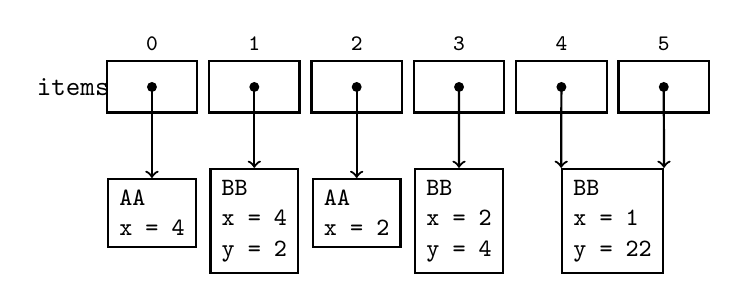
\begin{tikzpicture}[
    cell/.style={rectangle, draw, thick, minimum width=1.15cm, minimum height=0.65cm, font=\ttfamily},
    obj/.style={rectangle, draw, thick, align=left, font=\ttfamily\small, inner sep=4pt}
]
    \node[font=\ttfamily\bfseries] at (-1.0, 0) {items};
    \foreach \i in {0,...,5} {
        \node[cell] (c\i) at (\i*1.3, 0) {};
        \node[font=\ttfamily\footnotesize] at (\i*1.3, 0.55) {\i};
    }

    \node[obj] (o0) at (0, -1.6) {\textbf{AA}\\x = 4};
    \node[obj] (o1) at (1.3, -1.7) {\textbf{BB}\\x = 4\\y = 2};
    \node[obj] (o2) at (2.6, -1.6) {\textbf{AA}\\x = 2};
    \node[obj] (o3) at (3.9, -1.7) {\textbf{BB}\\x = 2\\y = 4};
    \node[obj] (o4) at (5.85, -1.7) {\textbf{BB}\\x = 1\\y = 22};

    \foreach \i in {0,...,3} {
        \fill (c\i.center) circle (1.8pt);
        \draw[->, thick] (c\i.center) -- (o\i.north);
    }
    \fill (c4.center) circle (1.8pt);
    \fill (c5.center) circle (1.8pt);
    \draw[->, thick] (c4.center) -- (o4.north west);
    \draw[->, thick] (c5.center) -- (o4.north east);
\end{tikzpicture}
\end{english}
\end{center}

المُخرج:
\begin{boxCode}
\begin{english}
\begin{minted}{text}
x = 4
x = 4 y = 2
x = 2
x = 2 y = 4
x = 1 y = 22
x = 1 y = 22
\end{minted}
\end{english}
\end{boxCode}
\end{boxSolution}

\filbreak

\begin{boxSolution}[\texorpdfstring{سؤال $17$ امتحان $\mathrm{899271}$ سنة $2024$ - فرع ب}{سؤال 17 امتحان 899271 سنة 2024 - فرع ب}]
\textbf{ب.} تتبّع التغييرات باختصار:
\begin{itemize}[itemsep=0.25em]
    \item \textenglish{items[0].Foo();} $\leftarrow$ تضع $x = 3$ في \textenglish{items[0]}.
    \item \textenglish{items[1].Goo();} $\leftarrow$ تستدعي \textenglish{BB.Goo()} فتضع $y = 4 - 1 = 3$.
    \item \textenglish{((AA) items[3]).Goo();} $\leftarrow$ الربط المتأخّر يستدعي \textenglish{BB.Goo()} فتضع $y = 2 - 1 = 1$.
    \item \textenglish{items[4].Bar();} $\leftarrow$ تستدعي \textenglish{AA.Bar()} التي تستدعي \textenglish{BB.Goo()} فتضع $y = 1 - 1 = 0$ (ويشير إليها \textenglish{items[5]} أيضًا).
    \item \textenglish{temp = new BB(1)} ($x = 1, y = 2$)، ثمّ \textenglish{temp.Bar()} تجعل $y = 0$، وتُطبع: \textenglish{Temp: x = 1 y = 0}.
    \item \textenglish{temp.Bar(9)} تضع $y = 9 + 1 + 0 = 10$، ثمّ \textenglish{items[2] = temp}.
\end{itemize}

المُخرج الكامل للفرع ب:
\begin{boxCode}
\begin{english}
\begin{minted}{text}
Temp: x = 1 y = 0
x = 3
x = 4 y = 3
x = 1 y = 10
x = 2 y = 1
x = 1 y = 0
x = 1 y = 0
\end{minted}
\end{english}
\end{boxCode}
\end{boxSolution}
\fi
\filbreak
